%!TEX program = xelatex
\PassOptionsToPackage{table,svgnames}{xcolor}
\PassOptionsToPackage{french}{translator}
\documentclass[aspectratio=169,11pt]{beamer}

%----------------------------------------
% Packages
%----------------------------------------
%\usepackage[utf8]{inputenc}
\usepackage[T1]{fontenc}
\usepackage{translator}
\usepackage{lmodern}
\usepackage{hyperref}
\usepackage{xcolor}
\usepackage{listings}
\usepackage{amsmath}
\usepackage{amssymb}
\usepackage{mathrsfs}
\usepackage{array}
\usepackage{tabularx}
\usepackage{multirow}
\usepackage[justification=centering]{caption}
\usepackage{float}
\usepackage{standalone}
\usepackage{import}
% PGF-TikZ
\usepackage{pgf}
\usepackage{tikz}
\usepackage{pgf-umlsd}
\usepackage{pgfgantt}

%----------------------------------------
% Theme
%----------------------------------------

\usetheme{boxes}
\useoutertheme{infolines}
\usecolortheme{whale}%beaver
\usecolortheme{seagull}

% remove bottom line
\setbeamertemplate{footline}{}

% remove navigation symbols.
\beamertemplatenavigationsymbolsempty{}

%\setbeamercovered{transparent}

%----------------------------------------
% Informations
%----------------------------------------

\title{Construction d'objet paramétrique}
\subtitle{IN55}
\author{Julien Barbier, Jérôme Boulmier, Maxime Pinard}
\institute[UTBM]{Université de Technologie de Belfort Montbéliard}
\date[22/06/18]{22 Juin 2018}

%\keywords{}
\subject{IN55 Construction d'objet paramétrique}
%\logo{\includegraphics[width=0.12\textwidth]{logos/IN55}}

%----------------------------------------
% Configurations
%----------------------------------------

\graphicspath{{figures/}}

\AtBeginSection
{
	\begin{frame}<beamer>
		\vfill{}
		\centering
		\begin{beamercolorbox}[sep=8pt,center]{title}
			\Huge\insertsectionhead\par%
		\end{beamercolorbox}
		\vfill{}
	\end{frame}
}

%----------------------------------------
% Figures configuration
%----------------------------------------

\usetikzlibrary{shapes}
\usetikzlibrary{arrows.meta}
\usetikzlibrary{calc}
\usetikzlibrary{matrix}


\makeatletter
\let\@@magyar@captionfix\relax
\makeatother

%----------------------------------------
% Document
%----------------------------------------
\begin{document}
	\begin{frame}
		\titlepage
	\end{frame}
	% \begin{frame}{Sommaire}
	% 	\tableofcontents
	% \end{frame}
	\section{Section}
		\subsection{Subsection}
			\begin{frame}
				\frametitle{Title}
				\framesubtitle{Subtitle}
				\begin{block}{Block title}
					Block text
				\end{block}
				Text
				\begin{itemize}
					\item item
					\item item
				\end{itemize}
			\end{frame}
	\section{Conception et technologies utilisées}
		\subsection{Technologie utilisées}
			\begin{frame}
				\begin{itemize}
					\item OpenGL
					\item GLFW
					\item ImGUI
				\end{itemize}
			\end{frame}
		\subsection{UML}
			\begin{frame}
				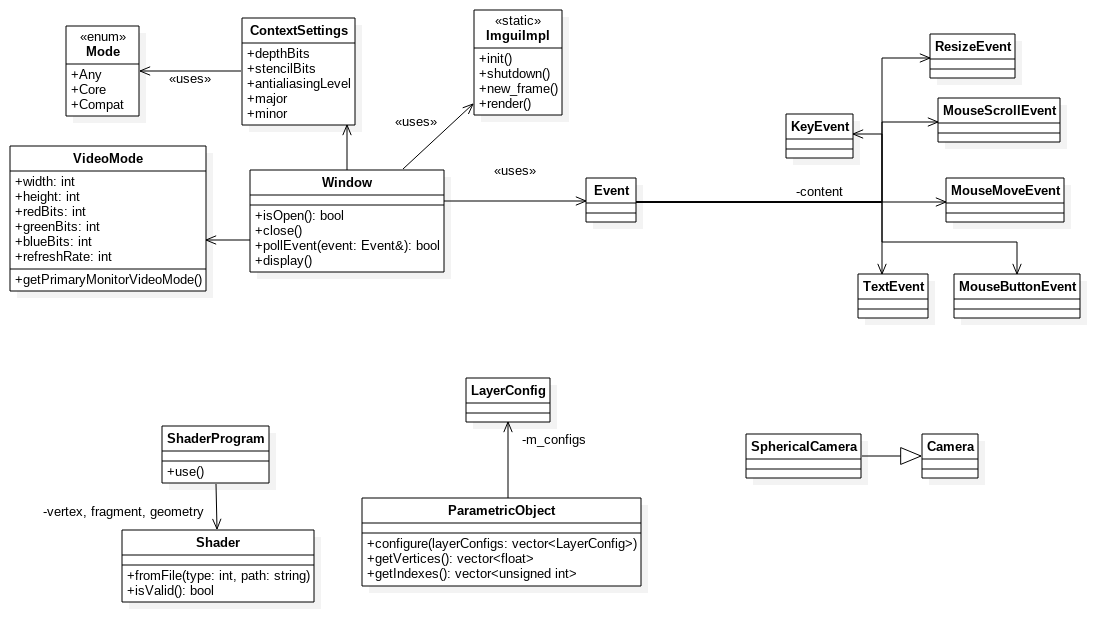
\includegraphics[width=\textwidth]{uml}
			\end{frame}
			\begin{frame}
				\centering%
				\resizebox{0.5\textwidth}{!}{\import{figures/}{seq_face_1.tex}}%
			\end{frame}
\end{document}
